To date, astronomers have observed over 2000 pulsars, these can be accessed
through the ATNF pulsar catalogue \citet{ATNF}. We can categorise the population
by their measured values of period $P$ and period derivative $\Pdot$. This is
done by plotting them in a $P - \Pdot$ diagram as shown
in figure \ref{fig: Period_PeriodDot}. Some of the pulsar varieties have been 
demarked in this plot and we now discuss their features. 

\begin{figure}[hb]
    \centering
    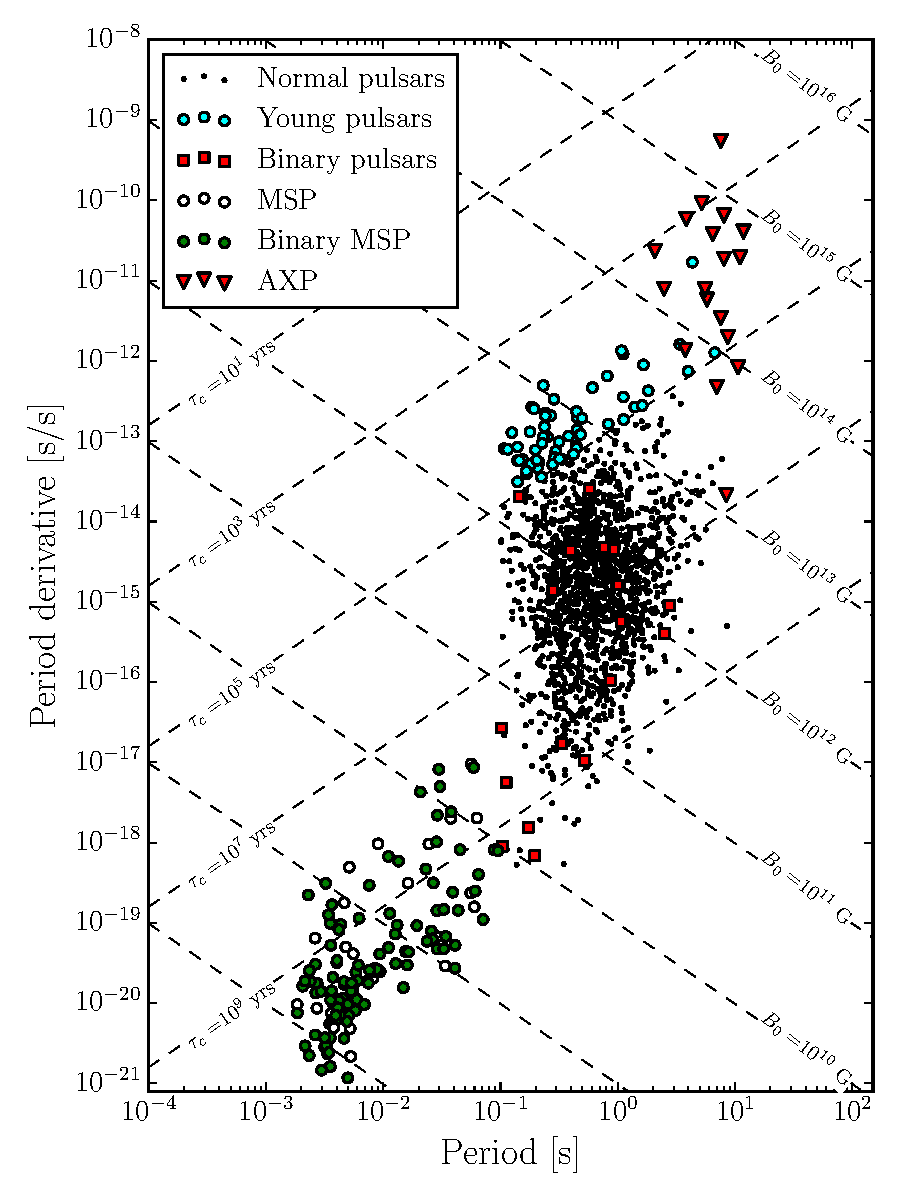
\includegraphics[width=0.6\textwidth]{Period_PeriodDot}
    \caption{Period - period diagram using data taken from the ATNF pulsar 
             catalogue \citep{ATNF}. Dashed lines show constant magnetic fields
         in units of Gauss and characteristic ages in units of years as described
     in section \ref{sec: rotation powered pulsars}}
    \label{fig: Period_PeriodDot}
\end{figure} 

The majority of pulsars, referred to as the `normal' pulsars, have a period of
$P=10^{-1}-10^{1}$~s. These can be described as \emph{rotation powered} pulsars
since the EM radiation is powered by the loss of rotational energy. As
described in section \ref{sec: rotation powered pulsars}, estimates can be made
for their characteristic age $\tau_{c}$ and surface magnetic field strength
$B_{0}$ based on a dipole spindown model. Constant lines of these quantities
are plotted in figure \ref{fig: Period_PeriodDot}. Of the normal pulsars, we
can identify the young pulsars as those for which $\tau_{c}<10^{5}$~yrs. Some
of these, such as the Crab and Vela, can be directly associated with their
supernova remnant from which they were formed \citep{Kaspi1996}. 

Some pulsars, known as binary pulsars, are found in orbit with other objects.
There is a wide variety of these objects but some notable examples include:
\begin{itemize}

    \item Two compact objects in a binary system: these provide unprecedented
        tests of general relativity. The
        the first such system found by \citet{Hulse1975} (which won the authors the 1993 Nobel prize)
        the perihelion advances at 4.2 degrees per year. More recently a double
        pulsar system \citep{KramerStairs2006} was found providing and even
        stronger test of general relativity since both objects could be timed.

     \item X-ray binary system: these are neutron stars which accrete matter
     from a nearby normal companion star. The in-falling matter during
     accretion is channelled by the magnetic field onto the magnetic poles.
     The gravitational potential energy released by the accreted matter is
     converted into X-ray radiation. In contrast to the rotation-powered
     pulsars, the EM radiation is therefore powered by accretion hence they are
     \emph{accretion-powered}. These are not included in the $P-\dot{P}$
     diagram of figure \ref{fig: Period_PeriodDot}.

\end{itemize}

A second smaller population of rotation powered pulsars exists with
$P<10^{-1}$~s, these are the \emph{millisecond pulsars} (MSPs). These special
class of pulsars are believed to start life as normal pulsars, but are then
spun-up through accretion from a normal star. During the accretion stage we
typically do not observe them as pulsars but as part of an X-ray binary system.
As a result many of the MSPs in figure \ref{fig: Period_PeriodDot} have a
binary companion.  Millisecond pulsars are typically very stable and are
frequently used in pulsar timing arrays.

Some pulsars are observed as sporadic bursts of energetic X-ray radiation,
these are known as anomalous X-ray pulsars (AXPs).  The neutron stars which are
thought to produce this emission have large magnetic fields $B_{0}\gtrsim
5\times10^{13}$; as a result they are named \emph{magnetars}. The high energy
radiation is thought to result from the decay of this magnetic field.


